\documentclass[a4paper]{article}
\usepackage{titling}
\usepackage[margin=1in]{geometry}
\usepackage{fullpage}
\usepackage{graphicx}



\title{\Huge \textbf{ID2090 ASSIGNMENT-4}}
\date{} 

\begin{document}

\begin{titlingpage}
\maketitle
\centering
\huge ARRHENIUS EQUATION
\thispagestyle{empty} 

\vspace*{\fill}

\begin{flushright}
\Large \begin{tabular}{@{}ll}
Name: Saisri.S \\
Roll No.: CH22B097 \\
Github userid: saisris
\end{tabular}
\end{flushright}
\end{titlingpage}


\newpage
\centering
\Huge ARRHENIUS EQUATION

\vspace{1cm}

\raggedright

\section{\textbf{Introduction:}}
\large



\ Arrhenius equation is a formula for the temperature dependence of reaction rates.\cite{ref=r1}.It was originally formulated by J.J. Hood on the basis of studies of the variation of rate constants of some reactions with temperature but the Swedish chemist Svante Arrhenius, for whom the equation is named, showed that the relationship is applicable to almost all kinds of reactions.It was introduced by him in 1889.


\section{\textbf{Equation:}}
\LARGE
$$k=Ae^{-(\frac{E_a}{RT})}$$
\large
Where,
\begin{itemize}
\item $k$ is the rate constant

\item $T$ is the absolute temperature

\item $A$ is the pre-exponential factor

\item $E_a$ is the activation energy for the reaction

\item $R$ is the universal gas constant

\end{itemize}

\section{\textbf{Arrhenius Plot:}}
$$k=Ae^{-(\frac{E_a}{RT})}$$

$$ln(k=Ae^{-(\frac{E_a}{RT})})$$

$$lnk=lnA+ln(e^{-(\frac{E_a}{RT})}$$
Solving the equation further,
$$lnk=lnA-{\frac{E_a}{RT}}$$
$$lnk=lnA-{\frac{E_a}{R}}(\frac{1}{T})\quad(1)$$

Comparing Eqn $1$ with $y=mx+c$

$m=-{\frac{E_a}{R}} , c=lnA$
\newpage
\begin{figure}[ht]
    \centering
    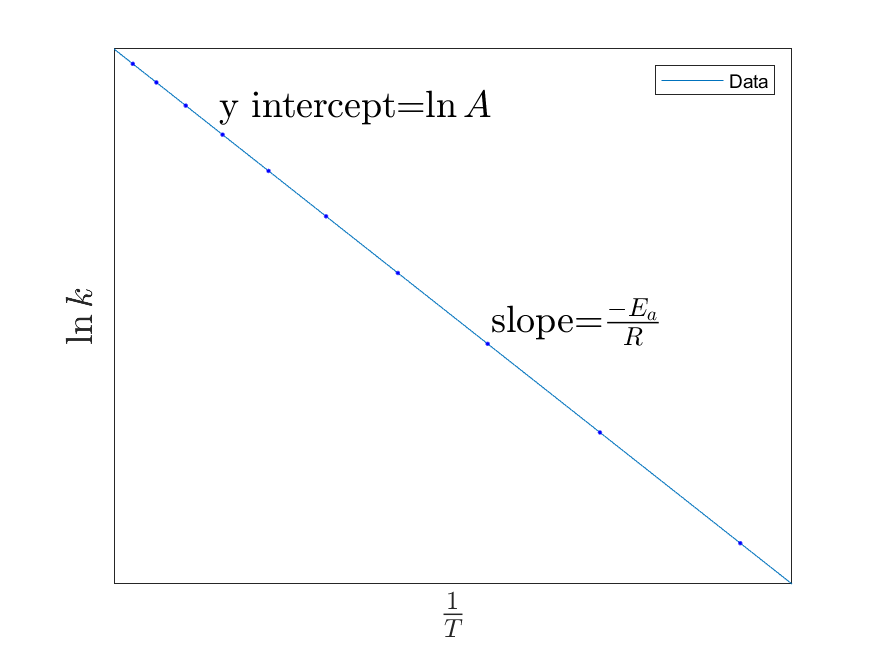
\includegraphics[width=0.5\textwidth]{ahhrenius.png}
    \caption{$lnk\quad v/s \quad \frac{1}{T}Plot$}
    \label{fig:example}
\end{figure}

\section{\textbf{ Pre-Exponential Factor (A):}}

The pre-exponential factor (A) in the Arrhenius equation – also called the frequency factor – is an important
variable which accounts for both the frequency of collisions between reactant molecules and the probability
that the molecules collide in the right geometry to produce an activated complex. The pre-exponential factor
can be evaluated both experimentally and through mathematical calculations. 
 \cite{ref=r2}.
The value of A is to be determined experimentally because it tends to assume several different values for several different reactions. It also depends on the temperature wherein the reaction takes place.

\section{\textbf{Activation Energy ($E_a$)}}
Activation energy is the minimum amount of energy that must be provided for compounds to result in a chemical reaction.In transition-state theory, the activation energy is the difference in energy content between atoms or molecules in an activated or transition-state configuration and the corresponding atoms and molecules in their initial configuration.Catalyst lowers the activation energy,increases the rate of reaction without being consumed in the reaction.

\section{\textbf{Modified arrhenius equation:}}
This is an extension of the simple Arrhenius equation in which the pre-exponential factor is proportional to $Tn$ where $T$ is the temperature and n a constant:~\cite{ref=r1}
$$k=AT^ne^{-(\frac{E_a}{RT})}$$

\section{\textbf{Conclusion:}}
Arrhenius equation enables the accounting of factors that have an effect on the rate of reaction and which is not possible to be determined by the rate law.It helps in finding the impact of energy barrier, frequency, temperature, the orientation of collisions, and presence of catalyst using the equation.
\newpage


\bibliography{references}
\bibliographystyle{plain}

\end{document}
\\



